%% LyX 2.0.6 created this file.  For more info, see http://www.lyx.org/.
%% Do not edit unless you really know what you are doing.
\documentclass[english,5p,sort&compress,times]{elsarticle}
\usepackage[T1]{fontenc}
\usepackage{color}
\usepackage{amsmath}
\usepackage{graphicx}
\usepackage{esint}

\makeatletter

%%%%%%%%%%%%%%%%%%%%%%%%%%%%%% LyX specific LaTeX commands.
%% Because html converters don't know tabularnewline
\providecommand{\tabularnewline}{\\}


%%%%%%%%%%%%%%%%%%%%%%%%%%%%%% User specified LaTeX commands.
%\usepackage{mathptmx}
%\usepackage{times}
%\def\thetable{\arabic{table}}
\usepackage{microtype}
\journal{Computational and Theoretical Chemistry}

\makeatother

\usepackage{babel}
\begin{document}

\title{Uranyl solvation by the three dimensional reference interaction site
model}


\author[tum]{Alexei Matveev\corref{corr}}


\ead{alexei.matveev@gmail.com}


\author[tum]{Bo Li}


\ead{fixme@abc.com}


\author[tum,crc]{Notker R�sch}


\ead{fixme@xyz.com}


\cortext[corr]{Corresponding author}


\address[tum]{Department Chemie, Technische Universit�t M�nchen, 85747 Garching,
Germany}


\address[crc]{Catalysis Research Center, Technische Universit�t M�nchen, 85747
Garching, Germany}
\begin{abstract}
We report an implementation of the three-dimensional reference interaction
site model (3D RISM) specifically describing the treatment of the
long-range Coulomb field of charged species represented by point charges
and/or distributed charge density. A comparison of 1D and 3D results
for atomic ions demonstrates the reasonable accuracy even for moderate
box size and grid resolution. In an application to uranyl aqua complexes
with 4\textendash{}6 explicit aqua ligands and an implicit bulk solvent
modeled by RISM, we demonstrate that the 3D technique is not susceptible
to the deficiencies of 1D technique exposed in our previous work {[}Li,
Matveev, Kr�ger, R�sch, \emph{Comp. Theor. Chem.} \textbf{1051}, p.~151,
(2015){]}. The 3D method eliminates the artificial superposition of
explicit aqua ligands and the RISM medium. It predicts essentially
the same values for uranyl and uranyl-water bond lengths as a state
of the art polarizable continuum model. We find that with the first
solvation shell treated explicitly, the observables are nearly independent
of the closure order. The water exchange activation barrier obtained
in a hybrid approach combining the quantum mechanical description
of the uranyl interaction within the first solvation shell and the
RISM model for the bulk solvent is in close agreement with the experimental
and the best theoretical estimates. \end{abstract}
\begin{keyword}
Reference interaction site model, uranyl, aqueous solution
\end{keyword}
\maketitle

\section{Introduction}

Thermodynamic and structural properties of the uranyl(VI) cation,
UO$_{2}^{2+}$, the most common uranium species in aqueous solution
are crucial for understanding its environmental chemistry as well
as chemical processes in radioactive waste disposal and recycling
of used nuclear fuel \citep{book:Morss06,book:Grenthe92,Silva95}.
Quantum mechanics (QM) and classical molecular mechanics (MM) simulations
provide the two complimentary ways to address microscopic structure
and energetics of solvated uranyl species. Till now, the most popular
strategy to combine the accuracy of QM methods and the complexity
of the statistical solvent description is to apply a polarizable continuum
model (PCM) to represent the effective electrostatic field of the
solvent, usually employed in combination with phenomenological corrections
for dispersion-repulsion interactions and cavity formation energy
using empiric parameters \citep{Tomasi05,Fuchs02}. The state of the
art PCM is owing its success in part to the conductor-like screening
model (COSMO) of electrostatic interactions \citep{Klamt95} and has
successfully been applied in various studies of uranyl complexes \citep{Fuchs02,Moskaleva04,Cao05,Shamov05,Gutowski06}.
On the other hand, there is a significant effort to improve the empirical
model potentials for MM simulations, such as molecular dynamics (MD)
or Monte-Carlo (MC) methods, that yield the most explicit statistical
solvent description \citep{Guilbaud93,Guilbaud96,Rai12,Pomogaev13,Kerisit13,Tiwari14}.
Though several studies \citep{Gordon00,hagberg05,Frick09,Tirler13}
attempt to combine QM and stochastic MM models such combinations will
inevitably lack the precise reproducibility  and efficiency of analytic
continuum models due to statistical sampling techniques. Yet more
demanding QM dynamic simulations \citep{Buehl05,Buehl06,Buehl11,Nichols08}
are restricted to comparably small numbers of solvent molecules. 

Meanwhile, the integral equation theories of molecular liquids \citep{book:Hirata03,book:Hansen06},
may provide sufficient accuracy at an affordable cost for simulating
chemical processes in solution by employing standard numerical methods
on contemporary hardware. Two approaches of this type are the reference
interaction site model (RISM) \citep{Chandler72,Hirata81,Hirata82,Kinoshita97}
and its three-dimensional generalization (3D RISM) \citep{Beglov95,Kovalenko98}
which provide the solvent structure in form of site-site radial distribution
functions (RDFs) or three-dimensional distribution functions of solvent
sites in an external (solute) field, respectively. Both 1D and 3D
theories provide variational expressions for the solvation energy
in the form of the excess chemical potential for several closure types
\citep{Singer85,Kast08} and, hence, intuitive expressions for the
first derivatives. The dielectrically consistent RISM (DRISM) \citep{Perkyns92}
was designed to compensate the error of the gas-like dielectric response
of RISM for electrolytes and ionic solutes \citep{Perkyns94,Chiodo07,Chuev08,Joung13}.

A correct handling of the electrostatic field of a charge distribution
requires additional care when periodic boundary conditions are employed
to simulate finite systems \citep{Makov95}. It was understood early
that the long-range asymptotes of the radial correlation functions
induced by Coulomb interactions in RISM need a separate treatment
as well \citep{Ng74}. For 3D RISM the few practical approaches include
the background charge correction technique \citep{Kovalenko00b},
monopole correction \citep{Kloss08b}, and an exact re-summation for
a superposition of gaussian charges \citep{Perkyns10}. In this work
we present a generalization of the exact re-summation technique for
arbitrary solute charge densities.

The integral equation theory has been combined with Hartree--Fock
electronic structure theory for self-consistent field calculations
(RISM SCF) in the pioneering work of Ten-no, Hirata, and Kato and
has been first applied to formaldehyde and carbonyl compounds in water
\citep{Tenno93,Tenno94}. An extension to 3D RISM SCF was developed
for density functional theory (DFT) \citep{Kovalenko99} and \emph{ab
initio} calculations \citep{Kloss08}. The analytical gradients for
the self-consistent combination of 3D RISM and DFT \citep{Gusarov06}
simplify explorations of free energy landscapes. Some of the recent
developments of hybrid approaches combining integral equation theories
and quantum chemistry are discussed in the recent review by Sato \citep{Sato13}.


In this work, we first describe the implementation of the 3D RISM
approach and a numerical treatment of the long-range Coulomb field
of the charged solute, Section~\ref{sec:methodology}, and then validate
the implementation by comparing the results of 1D and 3D techniques
for alkali and halide ions, Section~\ref{sec:simple-ions}. We further
evaluate the performance of the method for the uranyl(VI) dication
in aqueous solution represented by aqua complexes $[\text{UO}_{2}(\text{H}_{2}\text{O})_{n}]^{2+}$,
($n=4-6$), using a force field, Section~\ref{sub:MM+RISM}, and
a quantum mechanical representation of interactions within the first
solvation shell, Section~\ref{sub:QM+RISM}. We also compare the
results to those of PCM calculations. The activation barrier of water
exchange in the first solvation shell is analyzed in Section~\ref{sub:water-exchange}
using QM and MM models of interactions in the first solvation shell.



\section{Methodology \label{sec:methodology}}


\subsection{3D RISM equations}

In the 3D RISM approach, the solvent sites are exposed to an external
field of a solute of general shape. The solute-solvent interactions
are thus assumed to be pairwise, which in this formulation excludes
\emph{polarizable} solutes. Further, the interactions are usually
approximated by superposition of pairwise site-site contributions.
The 3D RISM equations operating with site-specific distributions can
be written in the following form \citep{book:Hirata03}:

\begin{equation}
\begin{cases}
h=\chi\ast c\\
h=c+t\\
h=f(-v+t)
\end{cases}\label{eq:rsim-h-c-t}
\end{equation}
Here $h$, $c$, and $t$ are the vectors of total-, direct-, and
indirect correlation functions $h_{\alpha}(\vec{r})$, $c_{\alpha}(\vec{r})$,
and $t_{\alpha}(\vec{r})$. All are dimensionless unknowns of the
equations that will be represented on a uniform grid of points. The
greek subscripts, such as $\alpha$, enumerate solvent interaction
sites. 

The solvent susceptibility $\chi$ in the first of the three Eqs.~\ref{eq:rsim-h-c-t}
is represented by its (square symmetric) matrix $\chi_{\alpha\gamma}(r)$
derived from the radial site-site correlation functions of the pure
solvent in 1D RISM equations for a specific temperature and solvent
number density $\rho$. \citep{book:Hirata03}. The star denotes the
convolution integral and the sum over corresponding matrix indices.
For that reason it is convenient to represent the solvent susceptibility
by its (dimensionless) Fourier image $\tilde{\chi}_{\alpha\gamma}(k)$
\citep{Chandler72,book:Hirata03}. The solvent susceptibility as a
function of either $r$ or $k$ is spherically symmetric by construction.

The second of the Eqs.~\ref{eq:rsim-h-c-t} introduces the indirect
correlation $t$ that is conveniently used in the closure relation
--- the third and last of Eqs.~\ref{eq:rsim-h-c-t}. Closure is a
local relation between the values of site potential $v_{\alpha}(\vec{r})$
and, in this case, the indirect correlation $t_{\alpha}(\vec{r})$
at each point $\vec{r}$ and the value of the direct correlation $h_{\alpha}(\vec{r})$
at this point. It is the only non-linear relation between the unknowns
$h$, $c$ and $t$ in Eqs.~\ref{eq:rsim-h-c-t}. The site-specific
potentials $v$ are measured in units of temperature and thus are
also dimensionless. For the purposes of this work we have chosen a
very specific, though popular, form of the closure which happens to
be a relation between $h$ and the sum $x=-v+t$ sometimes referred
to as a renormalized indirect correlation \citep{Kast08}:
\begin{equation}
f(x)=\begin{cases}
\mathrm{e}^{x}-1 & x\le0\\
\sum_{k=1}^{n}x^{k}/k! & x>0
\end{cases}\label{eq:closure-pse}
\end{equation}
In the limit of $n\to\infty$ one recovers the hypernetted chain (HNC)
closure. Another popular closure is obtained for $n=1$. It was proposed
by Kovalenko and Hirata (KH) for improving the numerical stability
of the equations \citep{Kovalenko99}. Higher order closures with
$n>1$ are referred to as partial series expansion closures of order
$n$ (PSE$n$). For consistency, we will also refer to the KH closure
as PSE1 in this work.

We used pair-wise interactions between solute and solvent sites $i$
and $\alpha$ to define the solute field: $v_{\alpha}(\vec{r})=\beta\sum_{i}u_{i\alpha}(|\vec{r}-\vec{r}_{i}|)$
where $\beta$ is the inverse temperature. Each potential $u_{i\alpha}$
is defined as the sum of the Coulomb interaction $u_{i\alpha}^{\text{C}}(r)=q_{i}q_{\alpha}a[f_{\text{CS}}(ar)+f_{\text{CL}}(ar)]$,
where we separated the singular short-range $f_{\text{CS}}(r)=\mathrm{erfc}(r)/r$
from the regular long-range $f_{\text{CL}}(r)=\mathrm{erf}(r)/r$
part, and a Lennard--Jones (LJ) type potential, $u_{i\alpha}^{\text{LJ}}(r)=\epsilon_{i\alpha}f_{\text{LJ}}(r/\sigma_{i\alpha})$
with a LJ form $f_{\text{LJ}}(r)=4(r^{-12}-r^{-6})$. Parameters of
the pair interactions were derived from site parameters using the
Lorentz--Berthelot rules \citep{book:Hirata03}. The Ewald range parameter
$a=1.2$~�$^{-1}$ is common for all site pairs. Further, to circumvent
numerical problems with singularities the primitive forms $f_{\text{CS}}(r)$
and $f_{\text{LJ}}(r)$ were regularized by substituting them with
quadratic functions $\bar{f}(r)=f(b)+f^{\prime}(b)(r^{2}-b^{2})/2b$
for $r<b$. For our systems at room temperature the results were almost
indistinguishable for finite $b\le0.5$ so that we settled with $b=0.2$
in this work.


\subsection{Free-energy surface}

The analytical expression for the excess chemical potential $\mu$
of an unstructured solute and the HNC closure has been derived by
Singer and Chandler (here in temperature units) \citep{Singer85}:
\begin{equation}
\mu_{\text{HNC}}=\rho\int d^{3}r\sum_{\alpha}\left[h_{\alpha}^{2}/2-c_{\alpha}-c_{\alpha}h_{\alpha}/2\right].\label{eq:chem-pot-hnc}
\end{equation}
A modification for the KH closure \citep{Kovalenko99} and a generalization
for the arbitrary closure of the form $h=f(x)$ with $x=-v+t$ are
available: 
\begin{equation}
\mu=\mu_{\text{HNC}}+\rho\int\sum_{\alpha}\phi(x_{\alpha})d^{3}r
\end{equation}
with $\phi(x)=f(x)-x-\int_{0}^{x}f(y)dy$ having particularly a simple
form for the PSE$n$ closures: $\phi_{n}(x)=-x^{n+1}/(n+1)!$ for
$x>0$ and zero otherwise \citep{Kast08}. In the case of the KH (PSE1)
closure the additional term $-x^{2}/2$ cancels the $h^{2}/2$ term
of the HNC integrand, Eq.~\ref{eq:chem-pot-hnc}, in the regions
where $x=h>0$. 

The analytical expression for the excess chemical potential is a path-independent
integral of the work required to ``switch on'' the external (solute)
field $v$ \citep{Singer85,Kast08}. This property leads to straightforward
expressions for derivatives of the chemical potential with respect
to parameters affecting the external field, such as the location of
solute sites. Such a derivative is an expectation value of the corresponding
force, $d\mu/ds=\int(dv/ds)gd^{3}r$, with $g=h+1$.

The free energy surface as a function of solute parameters $s$ is
constructed as a composite functional
\begin{equation}
G[n_{\text{e}},s]=E[n_{\text{e}},s]+\mu(s),
\end{equation}
where $E[n_{\text{e}},s]$ is the solute internal energy depending
on the solutes' geometric degrees of freedom $s$ and, in the case
of a QM solute, also on the electronic density $n_{\text{e}}$, but
not on the solvent site distribution functions $h$ \citep{Bo15}. 

The uranyl solvation energy is then estimated as\textcolor{green}{{}
}
\begin{eqnarray}
\Delta G_{\text{sol}} & = & G[\text{UO}_{2}(\text{H}_{2}\text{O})_{n}^{2+}]-nG[\text{H}_{2}\text{O}]-E[\text{UO}_{2}^{2+}]\label{eq:dG-sol-definition}
\end{eqnarray}
for $n\ge0$ explicit aqua ligands. Note that without proper statistical
sampling over the solute degrees of freedom $s$ this approximation
of the solvation energy, justified to some extent for sufficiently
rigid solutes, breaks for increasingly many explicit water molecules
outside of the tightly bound first solvation shell as $n\to\infty$.
Indeed, in a gedankenexperiment the difference $G[(\text{H}_{2}\text{O})_{n}]-nG[\text{H}_{2}\text{O}]$
for the above definition of $G$ applied to water droplets asymptotically
approaches $n(\bar{E}[\text{H}_{2}\text{O}]-G[\text{H}_{2}\text{O}])$
where $\bar{E}$ is the average configurational energy of a water
molecule which is about $-$9.9~kcal/mol \citep{Berendsen87,Mahoney00}
to be compared to the solvation energy of $-$6.3~kcal/mol derived
from the ratio of the equilibrium vapor/liquid concentrations \citep{Bridgeman64}.


\subsection{Numerical solution of 3D RISM equations}

Because of the highly non-linear closure relation, a single variable
fix point iteration scheme, $t^{(n+1)}=T[t^{(n)}]$, with $T[t]=(\chi-1)\ast c(t)$
and $c(t)=f(-v+t)-t$ as derived from the non-linear equation system,
Eqs.~\ref{eq:rsim-h-c-t}, is bound to diverge for all but the simplest
cases. To overcome the divergence problem we solve the reduced non-linear
problem $F[t]=T[t]-t=0$ using the Newton--Krylov non-linear solver
\citep{petsc-user-ref} with the analytic matrix-free Jacobian, $J[t]=\delta F/\delta t$,
occasionally preceded by a few Picard iterations.

The long-range field of a charged solute requires a special treatment
in the 3D case. All of the practical approaches, including the Ng
scheme \citep{Ng74}, separate the smooth asymptote $v_{\text{L}}$
of the site specific potential off the indirect correlation $t$ as
well as $-v_{\text{L}}$ off the direct correlation $c$ to operate
primarily with the short range counterparts $v_{\text{S}}$ , $c_{\text{S}}$,
and $t_{\text{S}}$. An iteration scheme for the new primary variable
$t_{\text{S}}$ (and the resulting non-linear problem) will look slightly
different, though:

\begin{eqnarray}
T_{\text{S}}[t_{\text{S}}] & = & (\chi-1)\ast c_{\text{S}}(t_{\text{S}})-\tau
\end{eqnarray}
with $c_{\text{S}}(t_{\text{S}})=f(-v_{\text{S}}+t_{\text{S}})-t_{S}$
and the only term that involves a long-range operand being the constant
``renormalization'' term $\tau=\chi\ast v_{\text{L}}$. This term
is the convolution of solvent susceptibility with the asymptotic potential. 

The low $k$ behavior of the asymptotic potential $v_{\text{L}}$
originates from the Coulomb potential and is, in general, singular.
With our choice of separation into short- and long-range parts it
reads 
\begin{equation}
\tilde{v}_{\text{L}}(\vec{k})=q\tilde{\varphi}(k)\tilde{n}(\vec{k})\sim4\pi qQ/k^{2}
\end{equation}
with $\tilde{n}(\vec{k})$ being the solute electric form factor,
$Q=\tilde{n}(0)$ being the net solute charge, $q$ being the vector
of the solvent site charges $q_{\alpha}$ and $\tilde{\varphi}(k)=4\pi k^{-2}\exp(-k^{2}/4a^{2})$
the Fourier transform of the long range potential function $\varphi(r)=\mathrm{erf}(ar)/r$.
A straightforward representation of this convolution operand on a
3D grid is thus problematic and should be avoided. The result of the
convolution, $\tau$, is of short range, though.

Indeed, the low $k$ behavior of another convolution operand, the
solvent susceptibility is regular 
\begin{equation}
\tilde{\chi}_{\alpha\gamma}(k)\sim\rho\kappa+\frac{1}{2}d_{\alpha\gamma}k^{2}
\end{equation}
with the limit for $k\to0$ being proportional to the solvent compressibility
$\kappa$ (here in temperature units) \citep{book:Hansen06}. More
importantly, this limit is the same for all site pairs $\alpha$ and
$\gamma$. Though not enforced, this property is obeyed in practical
calculations with reasonable accuracy. The second, $o(k^{2})$, term
is site pair specific and is in particular responsible for the dielectric
response of the solvent --- it is this term that is addressed by the
dielectric correction of the DRISM approach \citep{Perkyns92,Cummings81,Kovalenko00b}.
The result of the convolution, 
\begin{equation}
\tilde{\tau}_{\alpha}(\vec{k})=\tilde{n}(\vec{k})\left[\tilde{\varphi}(k)\sum_{\gamma}\tilde{\chi}_{\alpha\gamma}(k)q_{\gamma}\right]\sim2\pi Q\sum_{\gamma}d_{\alpha\gamma}q_{\gamma}\label{eq:tau}
\end{equation}
is regular assuming net neutrality of the solvent, $\sum_{\gamma}q_{\gamma}=0$,
which makes the compressibility term vanish. Note that the terms in
square brackets, $\tilde{\varphi}(k)\sum_{\gamma}\tilde{\chi}_{\alpha\gamma}(k)q_{\gamma}=:\tilde{\theta}_{\alpha}(k)$
(one per solvent site $\alpha$), are convolutions of spherically
symmetric functions neither of which is solute specific. The functions
$\tilde{\theta}_{\alpha}(k)$ are site-specific solvent properties
representing response to a unit (here gaussian-broadened) charge that
should be computed using 1D techniques, just as the solvent susceptibility
$\tilde{\chi}_{\alpha\gamma}(k)$ itself. In the 1D case our deliberate
choice of the self-inverse discrete sine transform of type IV (DST-IV)
as a basic operation eliminates the need to treat the singularities
at $r=0$ and $k=0$ as the discrete representation do not include
these points by construction \citep{FFTW05}. The solute part is the
electric form factor $\tilde{n}(\vec{k})$ of an arbitrary solute
charge distribution $n(\vec{r})$ with a low $k$ expansion including
all multipoles of the charge distribution; it is treated by regular
3D techniques.

A similar approach was applied before to a monopole field of the solute
\citep{Kloss08b} and to a superposition of gaussian charge distributions
\citep{Perkyns10}.  The argument line used above assumes the net
neutrality of the solvent species and is not directly applicable to
electrolytes, though even then the low $k$ behavior of a convolution
like in Eq.~\ref{eq:tau} can be assumed to be regular, cp.\ the
discussion of the background charge correction in Ref.~\citep{Kovalenko00b}.
An interpretation of Eq.~\ref{eq:tau} as a linear response of the
pure solvent distribution to a (weak) electrostatic field of the charge
distribution $n(\vec{r})$ offers an intuitive way to judge the range
assumptions for most solvent-solute combinations, cf.~Eqs.~\ref{eq:rsim-h-c-t}
for sound closures that fulfill $f(x)\sim x$ upon linearization.


\section{Computational details \label{sec:computational-details}}

To model uranyl solvation we employ the SPC/E water model \citep{Berendsen87},
modified as suggested by Pettitt and Rossky \citep{Pettitt82} by
addition of a Lennard--Jones (LJ) term for hydrogen atoms with $\sigma_{\text{H}}=0.4$~�
and $\epsilon_{\text{H}}=0.046$~kcal/mol (PR-SPC/E). For atomic
ions we adopted the coincident SPC/E water model (cSPC/E) with $\sigma_{\text{H}}=1.1658$~�
and $\epsilon_{\text{H}}=0.01553$~kcal/mol as proposed by Luchko
and Kovalenko \citep{Luchko10} in order to compare with published
results. The uranyl-water interaction parameters were derived from
the second model proposed by Kerisit and Liu to strengthen the uranyl\textendash{}water
interaction with the uranium charge of 3.5~\emph{e} (KL2) \citep{Kerisit13}.
For convenience the reader may refer to our previous work \citep{Bo15}
where we summarized the literal values for the charge and LJ parameters
of several force-fields.

All free energy calculations were carried out for the temperature
of 298~K, with the dielectric constant set to 78.4 and the solvent
particle density $\rho=0.0333295$~�$^{-3}$. These parameters correspond
to a pressure of 1~atm. The 3D domain was represented by a cubic
cell of $20^{3}$~�$^{3}$ and a Cartesian grid with 96$^{3}$ points
and a resolution of about 0.208~�. The radial grid used to precompute
and interpolate the solvent susceptibility and its contractions with
the Coulomb kernel for use in Eq.~\ref{eq:tau} was chosen with a
radial range of 40~� and 1536 points corresponding to a resolution
of about 0.026~�. 

All-electron QM calculations were carried out with the linear combination
of Gaussian-type orbitals fitting-functions density functional method
\citep{Dunlap90} as implemented in the parallel code ParaGauss \citep{ParaGaussV3.1}.
The atomic approximation \citep{Matveev08} to the second-order Douglas\textendash{}Kroll\textendash{}Hess
scalar-relativistic approach \citep{rev:roesch96} was used to account
for relativistic effects; this approximation was shown to be very
accurate for uranyl aqua complexes. We employed the gradient-corrected
exchange-correlation functional (generalized gradient approximation,
GGA) \citep{Goerling99,kochDFT}, as suggested by Becke and Perdew
(BP) \citep{Becke88,Perdew86c}. The Kohn\textendash{}Sham orbitals
were represented by flexible Gaussian-type basis sets, contracted
in a generalized fashion using atomic eigenvectors. For U, we used
a basis set of the size (24s, 19p, 16d, 11f), contracted to {[}10s,
7p, 7d, 4f{]}; O and H atoms were described by standard basis sets,
(9s, 5p, 1d) $\to$ {[}5s, 4p, 1d{]} and (6s, 1p) $\to$ {[}4s, 1p{]},
respectively. These basis sets and further computational details are
the same as in earlier studies on uranyl species \citep{Moskaleva04,Moskaleva06b,Moskaleva06a,Kremleva12b,Bo15}. 

We used a COSMO PCM solvation model for comparison \citep{Fuchs02},
with the cavity defined via an effective solvent radius of 1.4~�
and van der Waals radii of solute atoms as tabulated by Bondi \citep{Bondi64}
and scaled by 1.125 (except for hydrogen). We carried out the cavity
tessellation with the FIXPVA approach \citep{Su09,Kremleva12b} (fixed
points with variable areas) to obtain numerically stable energies
and forces \citep{Kremleva12b}. 

Geometry optimizations have been carried out using the quasi-Newton
method and the constrained minimization algorithm as implemented in
the utility package ParaTools \citep{Chaffey-Millar11,Nikodem13}.
In QM+RISM calculations of symmetric uranyl aqua complexes the U\textendash{}O
bonds were relaxed but constrained to have the same value by symmetry.
In the corresponding MM+RISM calculations uranyl was rigid with the
U\textendash{}O distances fixed to 179~pm motivated by earlier results
\citep{Moskaleva04,Cao05,Buehl05}. However, for a study of the water
exchange with MM+RISM we adopted a flexible uranyl model without symmetry
constraints and compared two sets of intra-molecular parameters \citep{Kerisit13,Tiwari14}
with unconstrained QM+RISM results. The two uranyl force field models
we employed differ only by uranyl equilibrium bond length and force
constants for stretching and bending modes. The SPC/E geometry of
explicit water ligands in the aqua complexes {[}UO$_{2}$(H$_{2}$O)$_{n}${]}$^{2+}$,
$n=4-6$, features an O\textendash{}H distance of 100~pm and an H\textendash{}O\textendash{}H
angle of 109.47$^{\circ}$. 


\section{Simple ions \label{sec:simple-ions}}

To verify our 3D RISM implementation for charged solutes, we performed
a comparison to 1D RISM results for mono-atomic alkali and halide
ions \citep{Joung13,Bo15} applying the cSPC/E water model \citep{Berendsen87,Luchko10}.
With moderate settings for the grid \textcolor{blue}{size} of $64^{3}$
points in total and a cubic box volume of $20^{3}$~�$^{3}$ we are
able to match the 1D results up to \textcolor{blue}{0.2}~kcal/mol
or better. \textcolor{blue}{With a 50\% larger box size at the same
grid density the agreement improves to 0.07~kcal/mol; a further increase
of the grid density by 50\% improves the results insignificantly.}
The accuracy is slightly better for small cations than for the larger
anions. The values are comparable to MD with SPC/E water and experimental
results. The agreement may be slightly improved by a correction proportional
to the molar volume of the solute \citep{Sergiievskyi14} as was demonstrated
in our previous work \citep{Bo15}.  

\begin{table}[t]
\begin{centering}
\caption{The solvation energy (excess chemical potential) for alkali and halide
ions by 3D and 1D RISM approaches with the cSPC/E water model. MD
and experimental values are also shown for comparison.$^{a}$ \label{tab:simple-ions}}

\par\end{centering}

\small\vspace{1ex}

\begin{centering}
\begin{tabular}{lrrrrrr}
\hline 
 & Li$^{+}$ & Na$^{+}$ & K$^{+}$ & Cl$^{-}$ & Br$^{-}$ & I$^{-}$\tabularnewline
\hline 
KH & $-$108.5 & $-$85.0 & $-$68.5 & $-$78.4 & $-$72.\textcolor{blue}{6} & $-$62.9\tabularnewline
KH$^{b}$ & $-$108.5 & $-$85.0 & $-$68.5 & $-$78.5 & $-$72.6 & $-$63.1\tabularnewline
HNC & $-$111.\textcolor{blue}{7} & $-$86.3 & $-$69.3 & $-$79.8 & $-$74.1 & $-$64.7\tabularnewline
HNC$^{b}$ & $-$111.7 & $-$86.3 & $-$69.3 & $-$79.9 & $-$74.2 & $-$64.9\tabularnewline
MD$^{c}$ & $-$113.3 & $-$88.4 & $-$71.0 & $-$89.3 & $-$82.7 & $-$74.4\tabularnewline
Exp$^{d}$ & $-$113.8 & $-$88.7 & $-$71.2 & $-$89.1 & $-$82.7 & $-$74.3\tabularnewline
\end{tabular}
\par\end{centering}

\vspace{1ex}\footnotesize

$^{a}$~Energies in kcal/mol. KH and HNC closure relations have been
used. 3D domain is $20^{3}$ �$^{3}$ / $64^{3}$ pts. $^{b}$~1D
RISM from Ref.~\citep{Bo15}. $^{c}$~MD with SPC/E water from Ref.~\citep{Joung08}.
$^{d}$~Ref.~\citep{Schmid00}.
\end{table}



\section{Uranyl aqua complexes \label{sec:uranyl-aqua-complexes}}


\subsection{MM+RISM \label{sub:MM+RISM}}

In this section we examine a combination of 3D RISM for bulk water
and a force field potential energy surface for the interactions of
uranyl and $n$ explicit water ligands for $n=4-6$. The complex with
$n=4$ features a missing equatorial ligand and demonstrates a qualitative
difference of the optimal structures obtained by minimizing the MM
and and MM+RISM expressions of the potential (free) energy. Similar
to the findings in our previous work, using the 1D RISM formalism
\citep{Bo15}, the MM+RISM combination features a vacancy in the equatorial
plane of the uranyl corresponding to the location of the missing water
ligand, Figure~\ref{fig:spatial-distribution-4w}. The MM potential
energy surface features a minimum at a $D_{4\text{h}}$-like structure
with four water ligands evenly distributed in the equatorial plane;
structures featuring a vacancy in the equatorial plane are by 13--15~kcal/mol
higher on that potential energy surface. The average U--OW bond in
the MM-optimized structure of 239~pm is slightly shorter than the
corresponding bonds of 240--242~pm of the structures optimized at
the MM+RISM level, Table~\ref{tab:mm-rism}. The shorter distances
indicate weaker steric ligand-ligand repulsions in the under-coordinated
gas-phase complex. Note, however, there is a non-obvious opposite
effect of shortening U--OW distances from 243--244~pm to 240~pm
in five-coordinated uranyl complexes after embedding a gas phase complex
into the RISM medium, Table~\ref{tab:mm-rism}. This could be an
indication of a partial screening of steric repulsions of the equatorial
ligands by the solvent of the second solvation shell in saturated
complexes, also observed in PCM calculations, see below.

The mechanism by which the MM+RISM model compensates for the missing
ligand is a local increase of the water density at the location of
the missing explicit ligand, Figure~\ref{fig:spatial-distribution-4w}.
Due to a notable width of the local distribution, both in equatorial
and apical directions and less so in radial direction the RISM representation
of the missing ligand is not an exact substitute for an explicit water
ligand. Indeed, there is a measurable difference of the average U--OW
distances between the complexes with 4 and 5 explicit waters in the
first solvation shell: 241--242~pm for $n=4$ and 240~pm for $n=5$,
Table~\ref{tab:mm-rism}. 

The strong localization of the solvent medium at the equatorial vacancy
leads to divergence of the RISM equations with the PSE3 closure. This
is manifested by the missing values in Table~\ref{tab:mm-rism}.
Results for the five-coordinated uranyl models, on the other hand,
are essentially independent of the closure choice. The bare uranyl
model, where the axial symmetry makes the localization issue less
severe, does converge for all three closures, though the results are
significantly affected by the closure choice --- the solvation energy
at the PSE3 level of theory is by 20~kcal/mol lower than at the PSE1
level. A different source of errors is the approximation of the solute
by a single structure minimizing the conformation free energy instead
of an ensemble at thermal equilibrium. Whereas this could be justified
to some extent for solutes with rigid intra-molecular and strong ligand
bonds, the weakly associated water molecules of the second solvation
shell need a better statistical treatment. The model with six explicit
waters with one of them in the second shell ($n=5+1$, Table~\ref{tab:mm-rism})
illustrates the point. Whereas the structure of the first solvation
shell is very similar for $n=5$ and $n=5+1$ explicit waters, the
solvation energy, computed by Eq.~\ref{eq:dG-sol-definition} is
by about 5~kcal lower in the latter case. This is likely an artifact
of a missing statistical sum over positions and orientations of the
second shell water molecule. Hence a successful model shall treat
the strongly bound aqua ligands explicitly as a part of the solute
and weakly associated or free-floating water as a RISM medium in order
to be numerically stable and closure independent. 

\begin{table}[t]
\caption{Average uranyl--water distance of the first solvation shell, $d$(U--OW),
and an estimate for the uranyl solvation energy, $\Delta G_{\text{sol}}$,
obtained using gas phase MM (GP) and MM+RISM models with PSE closures
of order $n=1-3$ (PSE$n$), see Eq.~\ref{eq:closure-pse}.$^{a}$
\label{tab:mm-rism}}
\small\vspace{1ex}

\begin{centering}
\begin{tabular}{llrrrr}
\hline 
$n$ &  & 0 & 5$-$1$^{b}$ & 5 & 5+1$^{c}$\tabularnewline
\hline 
$d$(U--OW) & GP & --- & 239 & 244 & 243\tabularnewline
 & PSE1 & --- & 241 & 240 & 240\tabularnewline
 & PSE2 & --- & 242 & 240 & 240\tabularnewline
 & PSE3 & --- & na$^{d}$ & 240 & 240\tabularnewline
$\Delta G_{\text{sol}}$ & GP$^{e}$ & --- & $-$233 & $-$272 & $-$295\tabularnewline
 & PSE1 & $-$363 & $-$382 & $-$392 & $-$397\tabularnewline
 & PSE2 & $-$379 & $-$389 & $-$392 & $-$397\tabularnewline
 & PSE3 & $-$383 & na$^{d}$ & $-$392 & $-$397\tabularnewline
\end{tabular}
\par\end{centering}

\vspace{1ex}\footnotesize

$^{a}$~Bond lengths in pm, energies in kcal/mol. $^{b}$~GP structure
is $D_{4\text{h}}$ but the RISM structures feature a vacancy in the
equatorial plane corresponding to the missing ligand, see Figure~\ref{fig:spatial-distribution-4w}.
$^{c}$~Five-coordinated structure with the sixth water in the second
shell. $^{d}$~Value not available due to divergence. $^{e}$~The
GP row shows binding energies of $n$ water molecules to a rigid uranyl
with $d$(U--O) of 179~pm. 
\end{table}
\begin{figure}[t]
\caption{Water oxygen distribution around the uranyl aqua complex with four
explicit water ligands. The isosurface corresponds to $h=2$. The
area around the missing equatorial ligand is characterized by values
of $h$ more than ten times as high. Other lopes of the isosurface
correspond to second solvation shell and feature $h<6$. \label{fig:spatial-distribution-4w}}


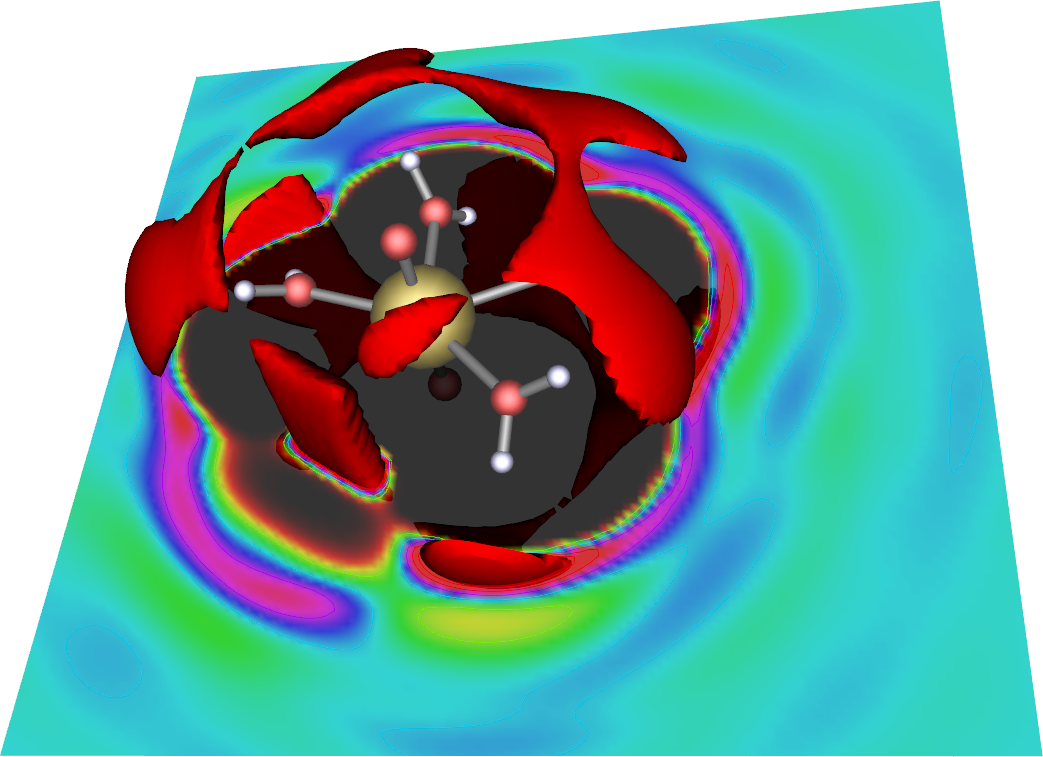
\includegraphics[width=1\linewidth]{4w}
\end{figure}



\subsection{QM+RISM \label{sub:QM+RISM}}

We use symmetric models of uranyl aqua complexes to compare PCM and
RISM representations of the solvent in QM calculations. The under-coordinated
species does not feature a vacancy in the first solvation shell. Instead
all water ligands are equivalent due to symmetry, also for the five-
and six-coordinated uranyl. These models feature an additional intra-molecular
degree of freedom, the uranyl bond length, in contrast to the MM models
discussed in the previous section where the uranyl bond was fixed
to a reasonable value. 

In our previous work exploring these models with 1D RISM \citep{Bo15}
we observed consistently longer U--O and U--OW bond lengths in QM+RISM
calculations in comparison to QM+PCM and experiment. We tentatively
attributed that to the excess coordination of uranyl, manifested by
the presence of a peak in the U--OW radial distribution at the distance
corresponding to the first solvation shell for models with explicit
ligands. This artifact is specific to 1D RISM and is not reproduced
in 3D RISM calculations, cp.\ Figure~\ref{fig:rdfs-vs-closure-5w}
showing no features at that separation and Figure~\ref{fig:rdfs-vs-closure-0w}.
The number integrals of 5.3, 6.2, and 6.4 for the first peak of U--OW
RDFs with PSE closures of order 1 to 3, respectively, for uranyl without
explicit aqua ligands (Figure~\ref{fig:rdfs-vs-closure-0w}) are
overestimated though.

Apart from the bare uranyl model the QM+RISM and QM+PCM results for
uranyl bond lengths of 179--180~pm agree in Table~\ref{tab:qm+rism-vs-qm+pcm}.
For the bare uranyl model the QM+RISM result is qualitatively better.
The QM+PCM predicts 174~pm for the uranyl bond length which is shorter
than for uranyl with just four water ligands. The QM+RISM results,
on the other hand, are around 179~pm being equally long (PSE1) or
even marginally longer by 0.3~pm and 0.7~pm for (PSE2 and PSE3,
respectively) than for four-coordinated uranyl (not visible in Table~\ref{tab:qm+rism-vs-qm+pcm}
due to rounding).  The effect of the RISM medium on the bond length
of the bare uranyl is thus comparable to that of the explicit water
ligands; the elongation of the uranyl bond by 7--8~pm corresponds
to 5--6~kcal/mol change in internal energy.

Another notable discrepancy between the PCM and 1D RISM results mentioned
in our previous work is also resolved by the 3D RISM approach: the
uranyl--water distances U--OW are consistently shorter in solvated
complexes than in the gas phase by measurable 4--6~pm. The 1D RISM
approach did not show this effect convincingly \citep{Bo15}. Again,
we interpret this effect of the medium as a screening of repulsive
ligand-ligand interactions in the first coordination shell by the
solvent. 

The magnitude of the uranyl solvation energy estimated with QM+RISM
models is comparable with that obtained in our previous work using
1D RISM. The estimates of $-$388 and $-$389~kcal/mol using the
standard model of hydrated uranyl with five explicit water ligands
vary only little with the closure order and agree well with $-$390~kcal/mol
from our previous work \citep{Bo15}. However, the relative order
of the estimates based on the four- and six-coordinated complexes
is not reproduced. The estimate of $\Delta G_{\text{sol}}$ based
on the four-coordinated complex is by $\sim$10~kcal/mol less negative
than the result of the standard model, Table~\ref{tab:qm+rism-vs-qm+pcm}.
This difference (but not the absolute numbers) is the same as the
PCM result, Table~\ref{tab:qm+rism-vs-qm+pcm}. However, this difference
is significantly larger than the value of 1.6~kcal/mol obtained using
1D RISM \citep{Bo15}, which is remarkably close to the free energy
difference corresponding to the relative weights of four- and five-coordinated
species determined from an average coordination number in a high-energy
x-ray scattering (HEXS) experiment \citep{Soderholm05}. Given the
limitations of 1D RISM exposed by the current 3D RISM approach we
interpret that past agreement as fortuitous.  $\Delta G_{\text{sol}}$
calculated from the six-coordinated $D_{3\text{d}}$ complex is by
4--5~kcal/mol more negative than the result of the standard model
with five explicit water ligands, Table~\ref{tab:qm+rism-vs-qm+pcm}.
The corresponding PCM difference is only 1~kcal/mol and of opposite
sign. It is likely that the limitations of the Eq.~\ref{eq:dG-sol-definition}
with the free energy of the complex approximated from a single symmetry-constrained
conformation is the source of this counter-intuitive ordering of estimates
for $\Delta G_{\text{sol}}$. For similar reasons the MM+RISM estimates
of the uranyl solvation energy using the models with different number
of explicit water molecules agree between each other no better than
to 3--5~kcal/mol even at the highest closure level, Table~\ref{tab:mm-rism}.
 Again, the solvation energy as determined by the QM+PCM model without
explicit water ligands ($n=0$) is by $\sim$100~kcal/mol off the
results obtained with $n=4-6$ explicit ligands, Table~\ref{tab:qm+rism-vs-qm+pcm}.
 The QM+PCM solvation energy of $-426$~kcal/mol given by the standard
five-coordinated uranyl model appears to be too low \citep{Moskaleva04}
in the view of most recent experimental estimate of $-369\pm15$~kcal/mol
\citep{Gibson05}. The corresponding QM+RISM solvation energy of $-389$~kcal/mol
is significantly closer to that interval. The properties in Table~\ref{tab:qm+rism-vs-qm+pcm}
obtained using the models with explicit water ligands separating the
uranyl di-cation and the RISM medium ($n=4-6$) hardly depend on the
closure order. This observation may justify the widespread use of
the lowest order PSE1 (KH) closure.  

\begin{table}[t]
\caption{Uranyl bond length, $d$(U--O), uranyl--water distance, $d$(U--OW),
and the uranyl solvation energy estimate, $\Delta G_{\text{sol}}$,
obtained using gas phase QM, QM+PCM and QM+RISM models.$^{a}$ \label{tab:qm+rism-vs-qm+pcm}}


\small\vspace{1ex}

\begin{centering}
\begin{tabular}{llrrrr}
\hline 
$n$ &  & 0 & 4$^{b}$ & 5$^{c}$ & 6$^{d}$\tabularnewline
\hline 
$d$(U--O) & GP & 172 & 177 & 177 & 178\tabularnewline
 & PCM & 174 & 179 & 179 & 180\tabularnewline
 & PSE1 & 179 & 179 & 179 & 180\tabularnewline
 & PSE2 & 179 & 179 & 179 & 180\tabularnewline
 & PSE3 & 179 & 179 & 179 & 180\tabularnewline
$d$(U--OW) & GP & --- & 242 & 249 & 253\tabularnewline
 & PCM & --- & 237 & 243 & 249\tabularnewline
 & PSE1 & --- & 237 & 243 & 248\tabularnewline
 & PSE2 & --- & 237 & 243 & 248\tabularnewline
 & PSE3 & --- & 237 & 243 & 248\tabularnewline
$\Delta G_{\text{sol}}$ & GP$^{e}$ & --- & $-$244 & $-$270 & $-$289\tabularnewline
 & PCM & $-$322 & $-$416 & $-$426 & $-$425\tabularnewline
 & PSE1 & $-$357 & $-$377 & $-$388 & $-$393\tabularnewline
 & PSE2 & $-$373 & $-$379 & $-$389 & $-$394\tabularnewline
 & PSE3 & $-$378 & $-$379 & $-$389 & $-$393\tabularnewline
\end{tabular}
\par\end{centering}

\vspace{1ex}\footnotesize

$^{a}$~Bond lengths in pm, energies in kcal/mol. Symmetric uranyl
aqua complexes {[}UO$_{2}$(H$_{2}$O)$_{n}${]}$^{2+}$, $4\leq n\leq6$
and a bare uranyl ($n=0$) are treated by QM while interactions with
the PR-SPC/E water solvent are treated by KL2 force field. $^{b}$~$D_{4\text{h}}$
structure. $^{c}$~$D_{5\text{h}}$ structure. $^{d}$~$D_{3\text{d}}$
structure. $^{e}$~The row shows binding energies of $n$ water ligands. 
\end{table}


\begin{figure}[t]
\caption{Radial distribution functions of the solvated uranyl without explicit
aqua ligands: U--OW (top panel, black), U--HW (top panel, gray), O--OW
(bottom panel, black) and O--HW (bottom panel, gray). Results employing
PSE1 closure are shown with the thick lines in the foreground. Results
employing PSE2 and PSE3 closures are displayed using thinner lines
in the background.  \label{fig:rdfs-vs-closure-0w}}


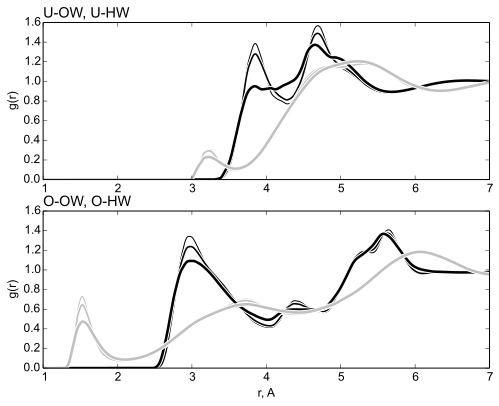
\includegraphics[width=1\linewidth]{fig2}
\end{figure}


\begin{figure}[t]
\caption{Radial distribution functions of the solvated uranyl complex with
five explicit water ligands in the equatorial plane. See Fig.~\ref{fig:rdfs-vs-closure-0w}
for explanation. \label{fig:rdfs-vs-closure-5w}}


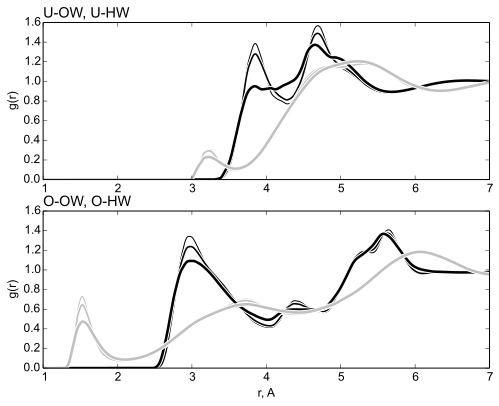
\includegraphics[width=1\linewidth]{fig3}
\end{figure}



\subsection{Water exchange \label{sub:water-exchange}}

By way of the Eyring equation the activation energy of aqua ligand
exchange process in the first solvation shell of uranyl computed from
the experimentally available water exchange rate estimate of 1.3$\times$10$^{6}$~s$^{-1}$
is about 9~kcal/mol \citep{Farkas00}. Many theoretical studies predict
much faster water exchange than the available experimental data suggests
\citep{Vallet01,hagberg05,Frick09,Nichols08,Kerisit10,Tiwari14}.
A simple way to obtain an estimate of the activation energy for the
water exchange may be the inspection of the U--OW potential of mean
force (PMF), $W(r)=-T\ln g(r)$, derived from the uranyl--water oxygen
RDF $g(r)$, Fig.\ \ref{fig:potential-of-mean-force}. In Table~\ref{tab:pmf-extrema}
we give the locations of the extrema of such PMF profiles, obtained
using the bare uranyl model and three different closure relations.
The activation energy estimated by 3D RISM as the PMF difference of
the first-shell minimum and the barrier top ranges from 3.4 to 5.2
kcal/mol, increasing with the closure order. The corresponding number
from the MD RDF is 4.4 kcal/mol. These values are comparable to the
5~kcal/mol derived from the residence time by Tiwari et al.~\citep{Tiwari14},
but significantly lower than the experimental estimate. The transition
between the first- and second solvation shells happens at U--OW separations
$r_{\text{b}}=309-324$~pm according to the radial PMF profiles.
Note that the one-particle radial PMF $W(r)$ provides no information
on the collective behavior of the water ligands during the water exchange,
thus it offers only limited insight into possible mechanisms. Also,
the RISM model for bare uranyl assumes a rigid linear geometry whereas
it was shown that uranyl bending essentially facilitates the water
exchange \citep{Tiwari14}.

Additional insight is provided by a three-dimensional PMF $W(\vec{r})=-T\ln g(\vec{r})$
given as $W(x,y)$ in Fig.\ \ref{fig:potential-of-mean-force-2d}
on a quarter of the axial plane with the uranium atom at the origin
and the uranyl oxygen on the $y$-axis. The location of the saddle
point  in Fig.\ \ref{fig:potential-of-mean-force-2d} corresponds
to a U--OW distance of 318~pm comparable with the respective PSE1
value in Table~\ref{tab:pmf-extrema}. The angle of attack for the
incoming/leaving water ligand estimated from that location is about
60$^{\circ}$ to the uranyl axis. This value is in good agreement
with the result of 61.8$^{\circ}$ from the transition state search
at Hartree--Fock level of theory with water solvent described by CPCM
model \citep{Vallet01}. A hypothetical water exchange in the equatorial
plane appears to be significantly hindered at room temperature. The
PMF values at the location of the saddle point and at the equatorial
minimum are 1.4~kcal/mol and $-1.7$~kcal/mol, respectively (PSE1).
Thus the activation barrier is about 3.1~kcal/mol which is only slightly
less than the estimate from the radial PMF, Table~\ref{tab:pmf-extrema}.
Again it is not possible to draw a conclusion on a collective behavior
of the incoming and leaving ligands from this one-particle property.

\begin{figure}[t]
\caption{Potential of mean force, $W(r)$, for U--OW distribution functions
obtained with PSE1, PSE2 and PSE3 closures (solid lines of decreasing
weight). The dashed line represents the MD result. \label{fig:potential-of-mean-force}}


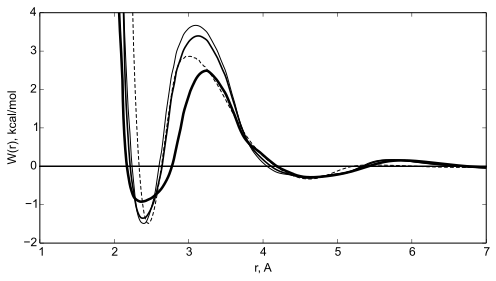
\includegraphics[width=1\linewidth]{pmf}
\end{figure}


\begin{table}[t]
\begin{centering}
\caption{PMF extrema $\{r_{i},W(r_{i})\}$,$^{a}$ and an estimate for the
water exchange activation energy, $\Delta W_{\text{ab}}=W(r_{\text{b}})-W(r_{\text{a}})$
extracted from the curves in Fig.\ \ref{fig:potential-of-mean-force}.
\label{tab:pmf-extrema}}

\par\end{centering}

\small\vspace{1ex}

\begin{centering}
\begin{tabular}{lrrrrrrr}
\hline 
 & $r_{\text{a}}$ & $W(r_{\text{a}})$ & $r_{\text{b}}$ & $W(r_{\text{b}})$ & $r_{\text{c}}$ & $W(r_{\text{c}})$ & $\Delta W_{\text{ab}}$\tabularnewline
\hline 
PSE1 & 236 & $-$0.9 & 324 & 2.5 & 465 & $-$0.3 & 3.4\tabularnewline
PSE2 & 238 & $-$1.4 & 313 & 3.4 & 462 & $-$0.3 & 4.8\tabularnewline
PSE3 & 240 & $-$1.5 & 309 & 3.7 & 461 & $-$0.3 & 5.2\tabularnewline
MD & 246 & $-$1.5 & 297 & 2.9 & 460 & $-$0.3 & 4.4\tabularnewline
\end{tabular}
\par\end{centering}

\vspace{1ex}\footnotesize

$^{a}$~Distances in pm, energies in kcal/mol. Locations $r_{\text{a}}$
and $r_{\text{c}}$ correspond to the minima of first- and second
solvation shells, respectively; $r_{\text{b}}$ is the highest point
of the barrier connecting the two minima. 
\end{table}


\begin{figure}[t]
\caption{Potential of mean force, $W(x,y)$, for the U--OW distribution functions
obtained with PSE1 closure. Here $x$ and $y$ are the radial and
axial displacements off the uranium atom. \label{fig:potential-of-mean-force-2d}}


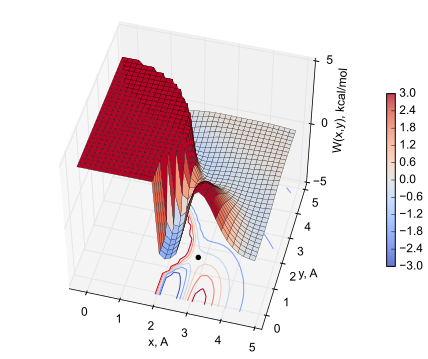
\includegraphics[width=1\linewidth]{pmf-2d}
\end{figure}


\begin{figure}[t]
\caption{Free energy profiles, $G(q)$, along the water exchange pathway using
two intra-molecular force fields with soft- and hard uranyl bending
modes (squares and diamonds, respectively). The QM+RISM profile is
represented by three stationary states (circles) connected by strait
lines to guide the eye. The reaction coordinate $q$ is the difference
of U--OW distances of two designated water molecules. \label{fig:free-energy-profiles}}


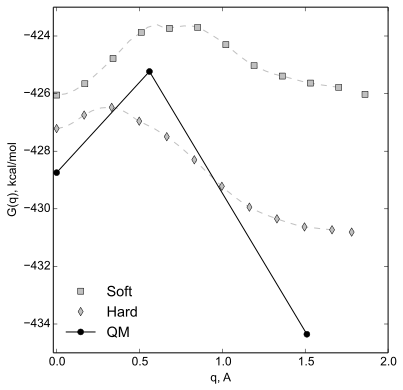
\includegraphics[width=1\linewidth]{profiles}
\end{figure}


To investigate the collective behavior of the ligands in the water
exchange process we need to treat the first solvation shell and the
incoming water molecule explicitly and also employ a flexible uranyl
model as it was shown that the uranyl bending may affect the exchange
rate \citep{Tiwari14}. The two intra-molecular force fields for a
flexible uranyl species we compare below differ primarily by the force
constant corresponding to the bending modes of uranyl and the equilibrium
bond length $d_{0}$(U--O). The force field here referred to as ``soft''
corresponds to the frequency of the bending mode of 159~cm$^{-1}$
and $d_{0}$(U--O) of 176~pm \citep{Tiwari14}. The alternative ``hard''
force field features a significantly higher frequency of the uranyl
bending mode of 393~cm$^{-1}$ and a somewhat too long a uranyl bond
 $d_{0}$(U--O) of 180~pm \citep{Kerisit13}. The bending vibration
in crystals and solution has been experimentally characterized by
frequencies in the range of 180--270~cm$^{-1}$ \citep{Denning76,Denning79,Toth81,Gal92}.
The DFT models with 5--6 explicit water ligands that we employ in
this and earlier works predict the bending frequency in this experimental
range \citep{Matveev08}. For the gas phase uranyl the standard DFT
predicts too soft a bending mode likely because of the self-interaction
error for $f$-electrons \citep{Ramakrishnan11} while hybrid DFT
and CCSD(T) estimate the bending frequency around 160--180~cm$^{-1}$
\citep{Jackson08}. In this light the force field with the ``soft''
bending mode appears to be a more reliable choice.

However, a comparison of the free energy profiles obtained with QM
and the two force field models of uranyl aqua complexes in RISM medium
reveals significant quantitative deficiencies for both force field
models. The Fig.~\ref{fig:free-energy-profiles} shows the three
free energy profiles along the reaction coordinate, $q=d(\text{U--OW}_{1})-d(\text{U--OW}_{2})$,
which is a difference of two uranium--water oxygen distances for incoming
and leaving water molecules. The QM+RISM profile is approximated by
just three stationary points. All of the three profiles feature an
intermediate metastable state at around $q=0$ roughly corresponding
to the six-coordinated $D_{3\text{d}}$-like uranyl aqua complex.
With the ``soft'' force field the uranyl species in the metastable
state is bent featuring an O--U--O angle of 155$^{\circ}$ and distances
to the two water ligands participating in exchange which are by about
15~pm longer than the distances to the other four water ligands;
the deviations from the $D_{3\text{d}}$ geometry for the other two
models, QM and ``hard'' force field, are less pronounced.  The
transition state approximated by the structure with the highest free
energy is characterized by $q>0.6$~� for both the QM and the ``soft''
uranyl models with the longest U--OW distance of 303~pm and 310~pm,
respectively. These distances are comparable to or slightly below
the estimates derived from the 1D and 3D PMFs above. The ``hard''
uranyl model, on the other hand, suggests a transition state with
a much shorter distance to the outermost water ligand of about 280~pm
and a shallow metastable state. This is likely due to the significantly
longer U--O bond of the solvated uranyl species of about 186~pm which
is more than 6~pm longer than those of the other models employed
here and in other works \citep{Tiwari14,Kerisit13} and should be
considered a deficiency of the parametrization.  In turn, the ``soft''
model does not convincingly show the preference for five-coordinated
uranyl with the sixth water in the second solvation shell over the
six-coordinated broken symmetry metastable structure. The QM and ``hard''
force field models predict the six-coordinated $D_{3\text{d}}$-like
state by 5.6~kcal/mol and 3.6~kcal/mol less stable than the five-coordinated
structure with an extra water in the second shell, respectively. The
presence of such a six-coordinated intermediate suggests an associative
two-step water exchange mechanism as one of the possibilities. This
is consistent with the findings of the other theoretical studies \citep{Tsushima07,Vallet01,Buehl06b,Rotzinger07,Tiwari14}
suggesting that the associative mechanism is more favorable than the
dissociative mechanism. 

The collective behavior of the uranyl aqua ligands is unspectacular
and can be described as a redistribution in the torus-shaped first
solvation shell roughly corresponding to the low PMF region, cp.~Figs.~\ref{fig:potential-of-mean-force}
and \ref{fig:potential-of-mean-force-2d}, while the sixth water molecule
enters or leaves the first solvation shell. The water exchange barrier
of 2.3 and 4.4~kcal/mol calculated with the ``soft'' and ``hard''
force field models, respectively, though not very far from the estimates
we obtained above from the PMF analysis, are significantly lower than
the 9.1~kcal/mol barrier of the QM+RISM model, Fig.~\ref{fig:free-energy-profiles},
which is in good agreement with the experimental estimate of 9~kcal/mol
\citep{Farkas00}.  A comparison of locations and orientations of
the second-shell explicit water which is connected by hydrogen bonds
to the two explicit aqua ligands of uranyl between the three models
suggests that the force field models may slightly underestimate the
strength and directional nature of the hydrogen bonds. This may explain
the low water exchange activation energy and the stability of the
six-coordinated metastable state relative to the structure with an
explicit water in the second shell, as predicted by the force field
models, Fig.~\ref{fig:free-energy-profiles}.

It should be noted that water activation energy barrier computed by
state of the art QM is sensitive to the choice of reaction path, level
of theory, and solvation model \citep{Tiwari14}. Tsushima \citep{Tsushima07}
reported the activation energy barriers of 10.1~kcal/mol and 4.8~kcal/mol
at the B3LYP level with the conductor-like polarizable continuum model
(CPCM) by considering the terminal states with one and two hydrogen
bonds, respectively. The latter value is close to the prediction of
4.5~kcal/mol in an earlier study \citep{Vallet01}, yet both are
lower than the experimental result. The comparison of PCM and a spherical
cavity self-consistent reaction field (SCRF) solvation models is reported
by Rotzinger \citep{Rotzinger07} using the complete active space
self-consistent field (CAS SCF) technique. The corresponding energy
barriers of the associative pathway are equal to 9.4~kcal/mol and
6.5~kcal/mol, respectively. Water exchange energy barrier based on
the thermodynamic sampling is also estimated by B�hl et.\ al \citep{Buehl06b}
using the \textit{ab initio} molecular dynamics (AIMD). Their result
of 6.7~kcal/mol is however lower than the experiment and the QM+RISM
value in this study. The good agreement of QM+RISM result with the
experiment and the best of other theoretical models indicates that
the RISM model provides a viable alternative solvation model for uranyl
aqua complexes in hybrid calculations and offers a reasonable accuracy
at an affordable cost. 


\section{Conclusions}

We presented a parallelized implementation of 3D RISM for charged
species and verified its performance on examples of atomic ions and
uranyl aqua complexes. We demonstrated that the method is not susceptible
to a deficiency exposed in our previous work for the 1D RISM technique
where an artificial superposition of explicit aqua ligands and the
RISM medium leads to an overestimation of effective uranyl--water
coordination and an excessive elongation of the U--O and U--OW bonds:
for the uranyl aqua complexes with 4--6 explicit ligands RISM predict
essentially the same structure of the first solvation shell as PCM.
A net effect of a missing explicit aqua ligand is qualitatively correctly
represented by an excess density of the RISM medium, leading to comparable
results for uranyl with 5 and 4 explicit water ligands. However, because
of the strong closure order dependence of the results and occasional
divergence for higher order closures a successful model will avoid
treating the first solvation shell of highly charged ions implicitly.
With a first solvation shell treated by explicit aqua ligands, the
observables are nearly independent of the closure order.

A hybrid approach employing two very different models of ion--water
interactions, \emph{ab initio} and force field, relies heavily on
the consistence of the two interaction models. Use of the KL2 force
field, featuring high charges of interacting sites of uranyl, as selected
in our previous study as the one predicting the highest uranyl solvation
energy, leads to a substitution of explicit QM aqua ligands by the
RISM medium far too easily for routine calculations to be practical.
Such artifacts affected the 1D RISM approach as well suggesting that
this particular QM+RISM combination may need to be revisited.

Nevertheless, by employing the 3D RISM model for the second solvation
shell and the bulk water, the hybrid QM+RISM model produces meaningful
structure of the first solvation shell and solvation energies competitive
to the state of the art PCM. By examining the water exchange activation
energy we demonstrated the usefulness of the hybrid QM+RISM models
to address properties that are not easily reproduced by pure force
field models. The activation energy is predicted too low with the
force field models, likely due to the misrepresentation of hydrogen
bonding. It is in remarkably good agreement with the experiment when
the hybrid QM+RISM model is employed.




\section*{Acknowledgments}

We thank Prof.~H.-J.~Bungartz and co-workers for valuable discussions
and Dr.~L.~Jager and Prof.~M.~Griebel for providing the source
of the BGY3D program package. BL is grateful for a fellowship by the
International Graduate School of Science and Engineering at Technische
Universit�t M�nchen. This work was partially supported by Bundesministerium
f�r Bildung und Forschung (grant No.\ 01RC1106A).

\bibliographystyle{elsarticle-num}
\bibliography{uo2}

\end{document}
